\documentclass[fleqn, a4paper, 12pt, twoside]{article}

\newcounter{recitationcount} %creates a new counter for recitation numbers (must be executed before exsheets is loaded)
\newcommand\recitation{\refstepcounter{recitationcount}}

\usepackage[counter-within = recitationcount]{exsheets} %question and solution environments
\usepackage{tasks}
\usepackage{amsmath, amssymb, amsthm} %standard AMS packages
\usepackage{esint} %integral signs
\usepackage{marginnote} %marginnotes
\usepackage{gensymb} %miscellaneous symbols
\usepackage{commath} %differential symbols
\usepackage{xcolor} %colours
\usepackage{cancel} %cancelling terms
\usepackage[free-standing-units]{siunitx} %formatting units
\usepackage{tikz, pgfplots} %diagrams
	\usetikzlibrary{calc, hobby, patterns, intersections, angles, quotes, spy}
\usepackage{graphicx} %inserting graphics
\usepackage{epstopdf} %converting and inserting eps graphics
\usepackage{hyperref} %hyperlinks
\usepackage{datetime} %date and time
\usepackage{ulem} %underline for \emph{}
\usepackage{xfrac, lmodern} %inline fractions
\usepackage{enumerate, enumitem} %numbered lists
\usepackage{float} %inserting floats
\usepackage[american voltages]{circuitikz} %circuit diagrams
\usepackage{pdflscape} %pages in landscape orientation
\usepackage{setspace} %double spacing
\usepackage{microtype} %micro-typography
\usepackage{listings} %formatting code
	\lstset{language=Matlab}
	\lstdefinestyle{standardMatlab}
	{
		belowcaptionskip=1\baselineskip,
		breaklines=true,
		frame=L,
		xleftmargin=\parindent,
		language=C,
		showstringspaces=false,
		basicstyle=\footnotesize\ttfamily,
		keywordstyle=\bfseries\color{green!40!black},
		commentstyle=\itshape\color{purple!40!black},
		identifierstyle=\color{blue},
		stringstyle=\color{orange},
	}
\usepackage{algpseudocode} %algorithms
\usepackage{algorithm} %algorithms

\newcommand\numberthis{\addtocounter{equation}{1}\tag{\theequation}} %adds numbers to specific equations in non-numbered list of equations

\theoremstyle{definition}
\newtheorem{example}{Example}
\newtheorem{definition}{Definition}

\theoremstyle{theorem}
\newtheorem{theorem}{Theorem}
\newtheorem{law}{Law}

\newcommand{\curl}{\mathrm{curl\,}}

\newcommand{\divergence}{\mathrm{div\,}}

\makeatletter
\@addtoreset{section}{part} %resets section numbers in new part
\makeatother

\newcommand\blfootnote[1]{%
	\begingroup
	\renewcommand\thefootnote{}\footnote{#1}%
	\addtocounter{footnote}{-1}%
	\endgroup
}

\renewcommand{\tilde}{\widetilde}

\RenewQuSolPair{question}[name=Recitation \therecitationcount\ -- Exercise]{solution}[name=Recitation \therecitationcount\ -- Solution]

\SetupExSheets{solution/print = true} %prints all solutions by default

%opening
\title{Numerical Analysis : Recitations}
\author{Aakash Jog}
\date{2015-16}

\begin{document}

\maketitle
%\setlength{\mathindent}{0pt}

\blfootnote
{	
	\begin{figure}[H]
		
\includegraphics[height = 12pt]{cc.eps}
		\includegraphics[height = 12pt]{by.eps}
		\includegraphics[height = 12pt]{nc.eps}
		\includegraphics[height = 12pt]{sa.eps}
	\end{figure}
	This work is licensed under the Creative Commons Attribution-NonCommercial-ShareAlike 4.0 International License. To view a copy of this license, visit \url{http://creativecommons.org/licenses/by-nc-sa/4.0/}.
} %CC-BY-NC-SA license

\tableofcontents

\newpage
\section{Instructor Information}

\textbf{Ron Levie}\\
~\\
E-mail: \href{mailto:ronlevie@post.tau.ac.il}{ronlevie@post.tau.ac.il}\\

\recitation
\section{Errors}

\begin{definition}[Error]
	The absolute error in representation is defined as
	\begin{align*}
		e_x & = x - \tilde{x}
	\end{align*}
	The relative error in representation is defined as
	\begin{align*}
		\delta & = \frac{x - \tilde{x}}{x}
	\end{align*}
\end{definition}

\begin{question}
	The dimensions of a field are measured.
	The length is measured to be $\tilde{x} = 800 \metre$, with an absolute error bounded by 16.
	The width is measured to be $\tilde{y} = 30 \metre$, with an absolute error $e_y$, such that $|e_y| \le 6$.\\
	\begin{enumerate}
		\item Find the approximate bounds for $|\delta_x|$ and $|\delta_y|$.
		\item Find the bounds on the absolute error in the calculated area of the field.
	\end{enumerate}
\end{question}

\begin{solution}
	\begin{enumerate}[leftmargin=*]
		\item
			\begin{align*}
				|\delta_x|            & = \frac{|e_x|}{|x|}    \\
                                                      & \le \frac{16}{|x|}     \\
                                                      & \approx \frac{16}{800} \\
                                                      & = 0.02                 \\
				\therefore |\delta_x| & \le 0.02
			\end{align*}
		
			\begin{align*}
				|\delta_y|            & = \frac{|e_y|}{|y|}   \\
                                                      & \le \frac{6}{|y|}     \\
                                                      & \approx \frac{6}{300} \\
                                                      & = 0.02                \\
				\therefore |\delta_y| & \le 0.02
			\end{align*}
		\item
			The measured area of the field is
			\begin{align*}
				\tilde{A} & = \tilde{x} \tilde{y} \\
                                          & = 800 \cdot 300       \\
                                          & = 240000
			\end{align*}
			The maximum area of the field is
			\begin{align*}
				A_{\textnormal{max}} & = (\tilde{x} + {e_x}_{\textnormal{max}}) (\tilde{y} + {e_y}_{\textnormal{max}}) \\
                                                     & = (800 + 16) (300 + 6)                                                          \\
                                                     & = 249696
			\end{align*}
			The maximum area of the field is
			\begin{align*}
				A_{\textnormal{min}} & = (\tilde{x} + {e_x}_{\textnormal{min}}) (\tilde{y} + {e_y}_{\textnormal{min}}) \\
                                                     & = (800 - 16) (300 - 6)                                                          \\
                                                     & = 230496
			\end{align*}
			Therefore,
			\begin{align*}
				|e_{x y}| & \le (A_{\textnormal{max}} - A_{\textnormal{min}}) \\
                                          & \le 9696
			\end{align*}
		\item
			\begin{align*}
				|\delta_{x y}| & = \frac{|e_{x y}}{|x y|} \\
                                               & \le \frac{9696}{|x y|}   \\
                                               & \le \frac{9696}{230496}  \\
                                               & \approx 0.042
			\end{align*}
	\end{enumerate}
\end{solution}

\subsection{Propagation of Error}

\begin{question}
	Let $\tilde{x}$, $\tilde{y}$ be approximations of $x$, $y$.
	\begin{enumerate}
		\item Find a formula for the absolute error in $x + y$ in terms of $e_x$ and $e_y$.
		\item Find a formula for $\delta_{x + y}$, $\delta_{x - y}$ in terms of $\delta_x$, $\delta_y$, $x$, $y$.
		\item
			Let $\delta = \max \{\delta_x,\delta_y\}$.
			Assuming $x,y > 0$, show
			\begin{align*}
				|\delta_{x - y}| & \le \frac{x + y}{|x - y|} \delta
			\end{align*}
	\end{enumerate}
\end{question}

\begin{solution}
	\begin{enumerate}[leftmargin=*]
		\item
			\begin{align*}
				e_{x + y} & = (x + y) - (\tilde{x} + \tilde{y}) \\
                                          & = (x - \tilde{x}) + (y - \tilde{y}) \\
                                          & = e_x + e_y
			\end{align*}
		\item
			\begin{align*}
				\delta_{x + y} & = \frac{e_{x + y}}{x + y} \\
                                               & = \frac{e_x + e_y}{x + y} \\
                                               & = \frac{x \delta_x + y \delta_y}{x + y}
			\end{align*}
			Similarly,
			\begin{align*}
				\delta_{x - y} & = \frac{e_{x - y}}{x - y} \\
                                               & = \frac{e_x - e_y}{x - y} \\
                                               & = \frac{x \delta_x - y \delta_y}{x - y}
			\end{align*}
		\item
			\begin{align*}
				|\delta_{x - y}| & = \left| \frac{x \delta_x - y \delta_y}{x - y} \right| \\
                                                 & \le \frac{|x| |\delta_x| + |y| |\delta_y|}{|x - y|}    \\
                                                 & \le \frac{x \delta + y \delta}{|x - y|}                \\
                                                 & = \frac{x + y}{|x - y|} \delta
			\end{align*}
	\end{enumerate}
\end{solution}

\begin{question}
	Find a formula for $\delta_{x y}$, in terms of $x$, $y$, $\delta_x$, $\delta_y$.
\end{question}

\begin{solution}
	\begin{align*}
		\delta_a             & = \frac{a - \tilde{a}}{a} \\
		\therefore \tilde{a} & = a (1 - \delta_a)
	\end{align*}
	Therefore,
	\begin{align*}
		\tilde{x} \tilde{y} & = \left( x (1 - \delta_x) \right) \left( y (1 - \delta_y) \right) \\
                                    & = x y (1 - \delta_x - \delta_y + \delta_x \delta_y)               \\
	\end{align*}
	Also,
	\begin{align*}
		\tilde{x} \tilde{y} & = x y (1 - \delta_{x y})
	\end{align*}
	Therefore,
	\begin{align*}
		\delta_{x y} & = \delta_x + \delta_y - \delta_x \delta_y
	\end{align*}
\end{solution}

\end{document}
